\documentclass[12pt, letterpaper]{article}  % standard LaTeX, 12 point type
\usepackage{amsfonts,latexsym}
\usepackage{amsthm, amssymb, amsmath}
\usepackage{fancyhdr} %Header package
\usepackage{lastpage}
\usepackage{graphicx}
\usepackage[margin=1in, dvips]{geometry} %1 inch margins.  Get rid of this line
                                         %if you prefer LaTex default formatting
\usepackage{hyperref} %Navigation in TOC and URLs in References
\usepackage{setspace}
\usepackage{float}
%\usepackage{appendix}
%\input{psfig.sty} % for imported eps files
\pagestyle{fancy}

%%% This LaTeX template is based on the Outstanding SIAM Award winning paper by the MIT team of Spann, Gulotta, and Kane in 2007. 
%%% Template by Andrew Spann, spann @(at) alum .(dot) mit .(dot) edu


% IMPORTANT: Set your team number in the header section after the summary



%%%%%%%%%%%%%%%%%%%%%%%%%%%%%%%%%%%%
%%%%%%%%%%%%%%%%%%%%%%%%%%%%%%%%%%%%
%%%%%%%%%%%%%%%%%%%%%%%%%%%%%%%%%%%%

%%%Preamble
%%  You can skip this part if you are not doing anything complicated


% This gets rid of LaTeX's tendency to wrap lines over-
% zealously.  The numbers are arbitrary.  Set it to over 9000 if you wish.
\hyphenpenalty=8000 \tolerance=1000


% Here are some suggested custom commands that you may find useful.  You can comment these out if you don't want them.  Most of these were suggested by MIT Professor Richard Stanley in his 18.091 mathematical exposition class.
\newtheorem{theorem}{Theorem}[section]
\newtheorem{proposition}[theorem]{Proposition}
\newtheorem{lemma}[theorem]{Lemma}
\newtheorem{corollary}[theorem]{Corollary}
\newtheorem{conjecture}[theorem]{Conjecture}

\theoremstyle{definition}
\newtheorem{example}{Example}[section]

% unnumbered environments:
\theoremstyle{remark}
\newtheorem*{remark}{Remark}
\newtheorem*{notation}{Notation}
\newtheorem*{note}{Note}

\newtheorem{thm}{Theorem}
\newtheorem{lem}[thm]{Lemma}
\theoremstyle{plain}
\newtheorem*{defn}{Definition}

% Richard Stanley's favorite macros
\newcommand{\CC}{\mathbb C} % blackboard math , for ``complex,'' etc
%\newcommand{\qed}{$\Box$}      % box  indicating end of proof.
% for a sequence of unnumbered displayed equations:
\newcommand{\beas}{\begin{eqnarray*}}
\newcommand{\eeas}{\end{eqnarray*}}
\newcommand{\bm}[1]{{\mbox{\boldmath $#1$}}} % for boldface math symbols


% More examples of LaTex macros, actually used in 2007 paper.
%\newcommand{\E}[1]{\textrm{E}\left[#1\right]}
%\newcommand{\V}[1]{\textrm{Var}\left[#1\right]}
%\newcommand{\SizeError}{2\%}
%\newcommand{\Cov}[2]{\textrm{Cov}\left(#1,#2 \right)}



% Blank parts of the header.  The rest is updated after the summary.
\lhead{ } \chead{ } \rhead{ } \cfoot{ }

%%%%%%%%%%%%%%%%%%%%%%%%%%%%%%%%%%%%%%%%%%%%
%%%%%%%%%%%%%%%%%%%%%%%%%%%%%%%%%%%%%%%%%%%%

\begin{document}

\ \vspace{0.3in} %%%%%%%%%%%%%  Summary  %%%%%%%%%%%%%%%%%%%%%%%%%%%%%

\begin{center}
\Large  %Your title here    \\
%Second line/subtitle if needed
\end{center}

\ \normalsize \\
%%% Type your summary here.  The summary is important, so leave enough time at the end to write it.  Remember to focus on your methodology and results in the summary, don't waste too much time on introduction material.  My 2007 summary is listed below in comments for your reference.











%%%%Spann, Gulotta, Kane 2007 summary for the Congressional Redistricting (gerrymandering) problem:

%We propose and evaluate two methods for determining congressional
%districts. The models are defined so that they only explicitly
%contain criteria for population equality and compactness, but we
%show through a detailed analysis that other fairness criteria such
%as contiguity and city integrity are present as emergent properties.

%In the Moment of Inertia Method, districts are created such that
%populations are within $\SizeError$ of the mean district size and
%the sum of the squares of distances between each census tract
%weighted by population size and the district's centroid is
%minimized.  We present a mathematical argument that this model will
%result in districts that are convex.

%In the Diminishing Halves Method, the state is recursively divided
%in half by a line that is perpendicular to the statistical best-fit
%line describing the region's census tracts.

%With the help of a Perl script we are able to parse US Census 2000
%data, extracting the latitude, longitude, and population count of
%each census tract. By parsing data at the census tract level instead
%of the county level, we are able to run our model with high
%precision.  We run our algorithms on census data from the states of
%New York as well as Arizona (small), Illinois (medium), and Texas
%(large).

%We compare the results of our methods to each other and to the
%current districts in the respective states.  Both our algorithms
%return districts that are not only contiguous but also convex, aside
%from borders where the state itself is nonconvex.  We superimpose
%city locations on the district maps to check for community
%integrity. We evaluate our proposed districts with the Inverse Roeck
%Test, the Length-Width Test, and the Schwartzberg Test to obtain
%quantitative measures of compactness.

%The initial conditions do not greatly affect the Moment of Inertia
%Method.  We run additional variants of the Diminishing Halves Method
%and find that they do not improve over our normal method.
%\medskip

%Based on our results, we would like to recommend to states that
%\begin{itemize}
%\item District shapes should be convex.
%\item City boundaries and contiguity can be emergent properties, not explicit considerations.
%\item A good algorithm can handle states of different sizes.
%\item We recommend our Moment of Inertia Method, as it
%consistently performed the best.
%\end{itemize}



\newpage

%%%%%%%%%%%%%%%%%%%%%%%%%%%%%%%%%%%%%%%%%%%%%%

% IMPORTANT  !!!!!
% IMPORTANT  !!!!!
% SET YOUR TEAM NUMBER BELOW:

\lhead{Team 41747}  \rhead{Table of Contents} \doublespacing

%I'm using doublespacing.  If you don't want that, get rid of the tag above.

%Using LaTeX gives you a table of contents for free!
\tableofcontents
\ \\

%%% Uncomment/Change the appendices below as relevant:
%\textbf{Appendix A: Full-Page Plots}\\
%\textbf{Appendix B: Computer Code}


\newpage

% Having completed the summary, now we define the header
\setcounter{page}{1} \chead{Section \thesection}  \rhead{Page
\thepage\ of \pageref{LastPage}}



%%%%%%%%%%%%%%%%%%%%%%%%%%%%%%%%%%%%%%%%%%%%%%%%%%%%%%%%%%%%%%%%

\section{Problem Restatement}\label{sec:restate}
%% One quick paragraph describing the problem and foreshadowing your approach.


Pursuit of a lost plane:

The disappearance of flight MH370 kindled a long debate and serious introspection. The methods used for hunting the plane came into serious questioning when even after months, the searchers were no closer to discovering the plane or its debris. 
The problem asks to Build a generic mathematical model that could assist "searchers" in planning a useful search for a lost plane feared to have crashed in open water such as the Atlantic, Pacific, Indian, Southern, or Arctic Ocean while flying from Point A to Point B. Like in the case of MH370, we arent receiving any signal from the plane that is feared to have crashed. 

The challenge in building a search model is the variation in Plane sizes and the different search techniques used. The problem requires to account for both.


%%%%%%%%%%%%%%%%%%%%%%%%%%%%%%%%%%%%%%%%%%%%%%%%%%%%%%%%%%%%%%%%%%%%
%%% Uncomment if needed
\section{Terminologies and Conventions}\label{sec:terms}

\begin{itemize}
\item \textbf{SAR}. Search-And-Rescue.

\item \textbf{MTOW}. Maximum Take Off Weight.

\item \textbf{$\tilde{r}$}. Distance between point of last contact and point of incident.

%and so on

\end{itemize}

%%%%%%%%%%%%%%%%%%%%%%%%%%%%%%%%%%%%%%%%%%%%%%%%%%%%%%%%%%%%%%%%%%%%

\section{Assumptions and their Justifications}\label{sec:assumptions}

\textit{\textbf{About the Search Domain and the Missing Aircraft}}
\begin{itemize}
\item \textbf{The search domain is a $500$km by $300$km rectangle of unobstructed ocean.} This rectangle would cover the whole uncertainty range based on 
the last known state of the lost aircraft for an interval of 15 minutes to 1 hour based on INMARSAT's "Log-on Interrogation" old and newly recommended standards in light of the MH370 accident\textbf{[citation]}.
\item \textbf{The missing aircraft is assumed to be still in this domain at $t=0$.} Although escaping the domain at a later time is allowed.
\item \textbf{The SAR targets remain clustered.} This means that the targets always stay in the same $20$km by $15$km cell on the coarse grid. This assumption is valid as long as the search plan is initiated close to the incident and no serve weather condition causes disturbances.
\item \textbf{There are buoyant indicator of target location at all time.} Since no underwater search is performed, we assume that either our SAR objective (e.g. survivors, life rafts, parts of crashed debris) remain buoyant throughout our search planning, or our sensor can detect signs of the objectives 
\item \textbf{The local trajectory of concern is straight}. In addition to the obvious smoothness arguments, it is always possible to apply a conformal transform on the entire search domain to obtain a solution based on a curved trajectory.

\item \textbf{No banking maneuver was made from incident to crash.} This is reasonable for that even in the worse case of gliding due to single engine failure, the average time from initial to of roughly $11$ minutes\textbf{[Citation or see derivation later]}. And this time is not long enough to cause trajectory deviations across different search cells.
\item \textbf{Hijacking or on-board navigation system only problems are not the cause of the incident}. Although hijacking incidents account for nearly $20$\% of all accidents in past 50 years \textbf{Citation!}, SAR plane (or vessel) detectors are largely useless in finding a cruising rouge plane. Also see problem restatement.
\item \textbf{The missing aircraft can be accurately modeled as either G280, Boeing 737-900ER, or Airbus 380.} These three types of aircraft are well-known representatives of small private/business jets, medium range commercial flights, and large international flights. Cruise speed and other aircraft form factors (e.g. Lift to Drag ratio) are derived based on this assumption.
\item \textbf{The crash radius of the aircraft is only a function of the cause of the incident and the type of the aircraft.} In addition, we assume that the historical distribution of the cause of the accidents is a reasonable prior for the current incident at hand, and it is it is invariant with respect to the type of the aircraft\footnote{We do not have an aircraft aficionado at hand to sift through and separate the accident records based on size}.
\item \textbf{Aircraft is operating at MTOW}. Assuming they have cargo and passengers 
\item \textbf{Cruise altitude of all types of aircraft is assumed to be the same}.  Describe/Justify.
%%%Add more items as needed
%%%Add more items as needed
\end{itemize}

\ \\
\textit{\textbf{About Debris Drifting}}
\begin{itemize}
\item \textbf{The local drift direction and speed can be accurately modeled as constant within each cell.} Operationally, the resolution of the cells can be adapted to actual drift data.
\item \textbf{Nothing outside the search domain drifts back into it.} This assumption only makes searching harder so good for us.
\end{itemize}

\ \\
\textit{\textbf{About the Search Agents}}
\begin{itemize}
\item \textbf{All agents are commanded and controlled by the central planner at each update interval.} No command and control overhead is assumed for the sake of simplicity.
\item \textbf{Agents arrive at the boundary of the search domain at $t=0$}.  Search agents are assumed to have arrived on the edge of the search domain at $t=0$.
\item \textbf{Unlimited bandwidth between search agent communications}.  This is necessary from a planning perspective as to ignore the less than pertinent issues with sensor fusion and coordination. Moreover, this factor is more than likely fixed by the hardware.
\item \textbf{Types of search agents considered are helicopter, fixed wing UAVs, and surface vessels.} Although the problem only mentions "search planes," it is very common to have sur
\item \textbf{Search agents use either magnetometer or camera as their main detector.}
\item \textbf{Search agents all have a lateral range function of a bivariate Gaussian as a function of their type, altitude, and speed.} Detection follows Koopman's Random search formula.
\item \textbf{The probability of false alarm is assumed to be $0$\%.} Lack of exact literature references, industry standard assumption [2013 book]. 
\item \textbf{The search agents have no knowledge of local drift direction.} Although modern planning softwares used by professional SAR entities (e.g. SARPOS by U.S. Coastal Guards) all have existing database to accommodate real-time ocean drifting, these data are often not precise, not to mention useless on a fictitious geography.
\item \textbf{Ignore refueling problems.} In operation, search agents can request refueling vehicles etc. and the time is not quite relevant.
\item \textbf{Agents move either horizontally or vertically.} In operation, search agents can request refueling vehicles etc. and the time is not quite relevant.

%%%Add more items as needed
\end{itemize}


%%Uncomment below if you want to begin the next section on a newpage:
%\newpage

%%%%%%%%%%%%%%%%%%%%%%%%%%%%%%%%%%%%%%%%%%%%%%%%%%%%%%%%%%%%%%%%%%%%

\section{Literature Review}\label{sec:litrev}

%% Maybe this isn't relevant to your paper or you want to just name this section as "INTRODUCTION".  There's a bit of flexibility as to what you can do now, so name this and the next few sections in whatever way fits the flow of your paper.  If convenient, I personally like to give a bit of scholarly journal background in some of my papers, but we don't do that every year depending on how weird the problems are.

1983 paper

2013 probablitic search book




%%Uncomment below if you want to begin the next section on a newpage:
%\newpage

%%%%%%%%%%%%%%%%%%%%%%%%%%%%%%%%%%%%%%%%%%%%%%%%%%%%%%%%%%%%%%%%%%%%

\section{Criteria for Optimal Solution}\label{sec:measure}

%% The problem usually doesn't give you a very specific definition for what the ``best'' solution is, so you should clearly explain it.  Feel free to rename this section something more relevant or use a different style and structure for the paper, just make sure you fulfill the goal of defining what the ``best'' solution looks like.

In real life the only success criterion is whether we can find the target and how long it takes to do so.

%\newpage

%%%%%%%%%%%%%%%%%%%%%%%%%%%%%%%%%%%%%%%%%%%%%%%%%%%%%%%%%%%%%%%%%%%%
\section{Describe Your Method}\label{sec:mainmethod}
%% (Change the section title of course)

%% Describe your mathematical model and list all relevant equations.  Remember to make your paper easy to skim by placing variable definitions by all equations.  We prefer to use actual words for variables if that variable will only be used once or twice.  Don't use Greek letters unless your variable is directly analogous to what a Greek letter usually means in math or physics.  Feel free to write important sentences \textbf{in bold} to make your paper easier to skim.


\begin{center}
	\begin{figure}[H]
		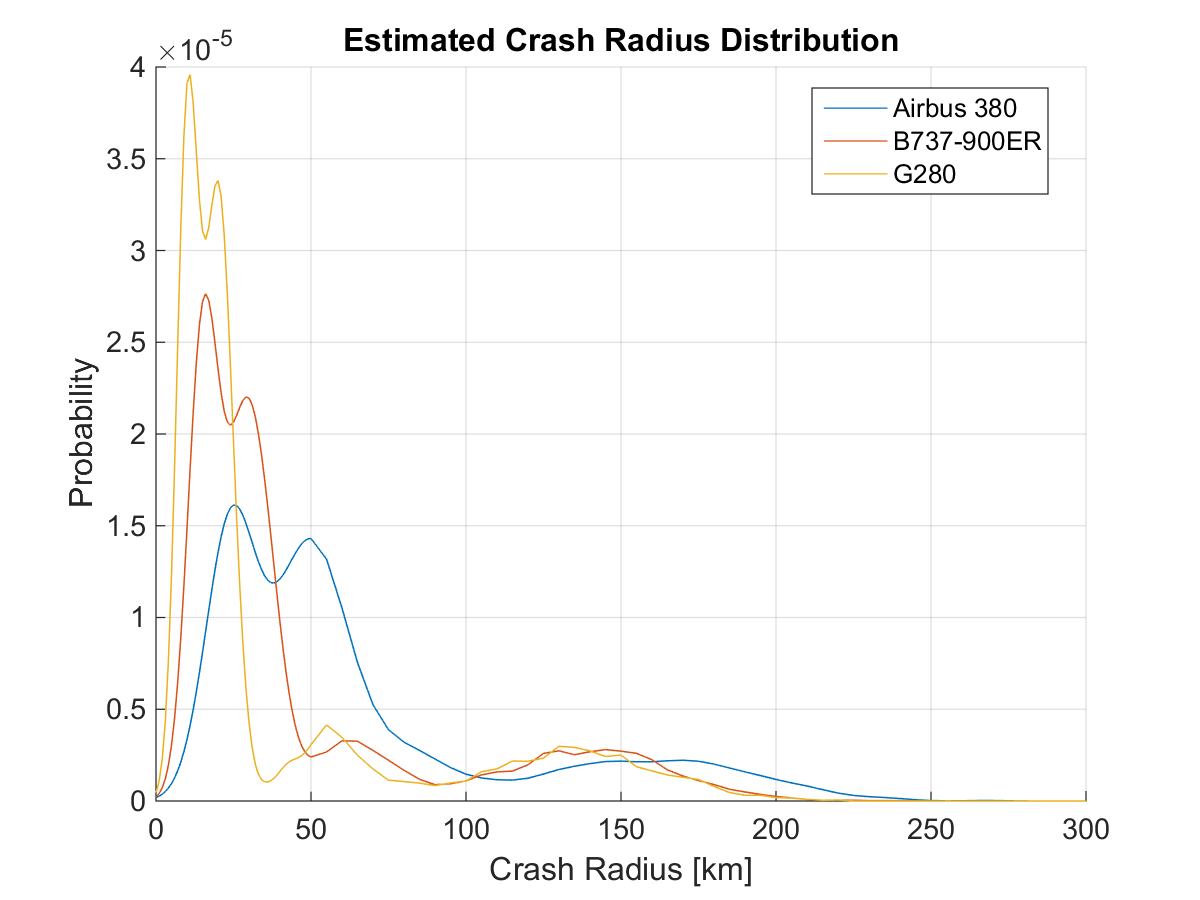
\includegraphics[width=0.9\linewidth]{simulation/CrashRadiusExplain.png}
		\caption{Estimated Crash Radius Distribution of three types of missing aircraft}
		\label{fig:CrashRadius}
	\end{figure}
\end{center}


\subsection{Description}\label{subsecmeth:desc}

%% Maybe you want to split this section into subsections.  Just suggesting things here.  Change as you see fit.  
%% By the way, you don't have to fill out the \label{}'s if you don't want to.  They're so you can \ref{} in the middle of the paper then move entire sections around later without breaking your numbering.


\subsection{Mathematical Interpretation}\label{subsecDist:math}

%% Here's quick lesson on equations if you need it:


\begin{center}
	\begin{figure}[H]
		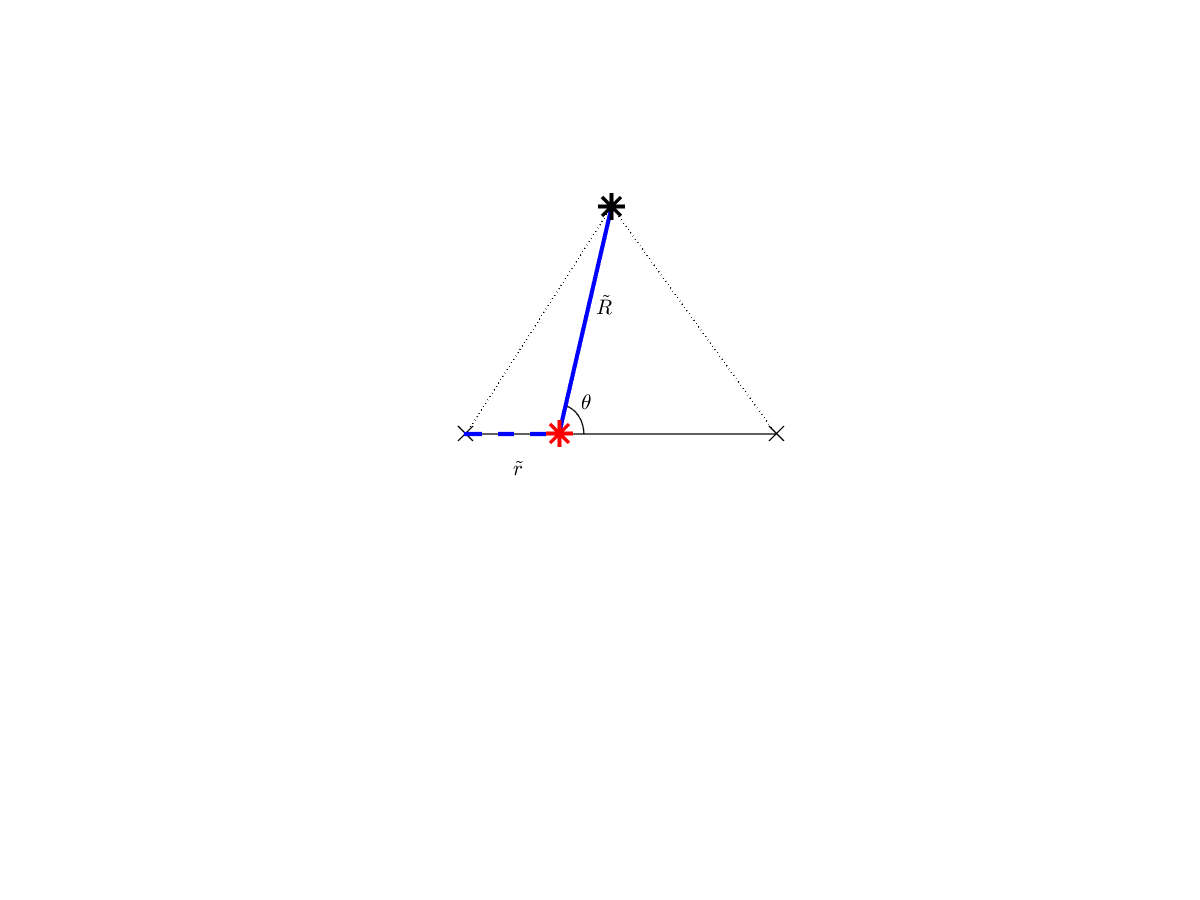
\includegraphics[width=0.9\linewidth]{simulation/LocationDensityExplain.png}
		\caption{Estimated Crash Radius Distribution of three types of missing aircraft}
		\label{fig:CrashRadius}
	\end{figure}
\end{center}

%%%% A standard numbered equation that you can later \ref{eqn:firstequation}

%\begin{equation}\label{eqn:firstequation}
% Type equation as if it were in between $ $ but you don't need the $.
%\end{equation}



%%%% Use & to split columns in align mode.  The * is optional, makes the equation not have a number.  You can have as many &'s per line as needed.

%\begin{align*}
%Left hand side   &   = Right hand side  \\
%                 &   = Right hand side on line below it\\
%                 &   = Final right hand side
%\end{align*}



\subsection{Comparison to Most Interesting Literature Paper}\label{subsec:hess}

%% Once again, change the sections as you see fit.  

%% Other command suggestions:
%\begin{lem}\label{biglem}
%\end{lem}

%\begin{proof}[Proof of Theorem \ref{algtheorem}]
%\end{proof}

%\section{}\label{labelme}

UAV paper

Current SARPOS system (particle filter)

%\newpage

%%%%%%%%%%%%%%%%%%%%%%%%%%%%%%%%%%%%%%%%%%%%%%%%%%%%%%%%%%%%%%%%%%
\section{Comparison to a "Steepest Decent" Search Plan}\label{sec:greedyalg}

%%% Besides your main model, always have a ``control'' algorithm to compare to.  It's even better if you can think of an extra ``good'' algorithm as well.  



also multiple agent/single agent etc.




%\newpage

%%%%%%%%%%%%%%%%%%%%%%%%%%%%%%%%%%%%%%%%%%%%%%%%%%%%%%%%%%%%%%%%%%
\section{Experimental Setup}\label{sec:experiment}
%% State clearly what you are testing.  State your input data and what probability distributions were used in generating it.  Talk a little bit about the implementation of your program (language, if something works a bit differently than the mathematical description you already gave them).  Split into subsections as needed.

grid cell size


%\newpage

%%%%%%%%%%%%%%%%%%%%%%%%%%%%%%%%%%%%%%%%%%%%%%%%%%%%%%%%%%%%%%%%%%
\section{Results}\label{sec:results}

%% List and describe your simulation results.  Besides the main question that you are being asked, seek other naturally occurring inquiries motivated by the results. Split your results into subsections as appropriate.


%%Here's how you input figures.  You can reference figures with \ref{}.
%%If you don't care about captions or referencing, you only need the %%\includegraphics{} part.






%\newpage

%%%%%%%%%%%%%%%%%%%%%%%%%%%%%%%%%%%%%%%%%%%%%%%%%%%%%%%%%%%%%%%%%%
\section{Sensitivity to Parameters}\label{sec:sensitive}

%% As a test for robustness, tweak some of the parameters to your model to see if the results would be substantially impacted.  You might also want to ask some additional sanity check questions based on the data and answer them.

Probability of Escape sensitive to grid size. (manifestation of discretization error)


%\newpage

%%%%%%%%%%%%%%%%%%%%%%%%%%%%%%%%%%%%%%%%%%%%%%%%%%%%%%%%%%%%%%%%%%
\section{Strengths and Weaknesses}\label{sec:sandw}
%%  You can write most of this section before 100\% of your results are done if your coding is running a little behind.  It doesn't have to be exactly 5 bullet points, just whatever makes sense given your paper.


\textit{Strengths:}
\begin{itemize}
\item \textbf{simple effective}.  Description.
\item \textbf{Short bullet point}.  Description.
\item \textbf{Short bullet point}.  Description.
\item \textbf{Short bullet point}.  Description.
\item \textbf{Short bullet point}.  Description.
\end{itemize}
\ \\
\noindent \textit{Weaknesses:}
\begin{itemize}
\item \textbf{resolution/grid size}.  Description.
\item \textbf{renomalization/discretization error}.  Description.
\item \textbf{very simplified drift modeling}.  Description.
\item \textbf{Short bullet point}.  Description.
\item \textbf{Short bullet point}.  Description.
\end{itemize}






%%Uncomment below if you want to begin the next section on a newpage:
%\newpage

%%%%%%%%%%%%%%%%%%%%%%%%%%%%%%%%%%%%%%%%%%%%%%%%%%%%%%%%%%%%%%%%%%

\section{Conclusion}\label{sec:conclusion}

%%  Almost there!  Time to highlight your most important policy recommendations based on the data you observed.

%% A couple paragraphs summarizing everything, then big bullet points to finish:

\begin{itemize}
\item \textbf{Recommendation 1}.  Why the data says so.
\item \textbf{Recommendation 2}.  Why the data says so.
\item \textbf{Recommendation 3}.  Why the data says so.
\item \textbf{Recommendation 4}.  Why the data says so.
% Exact Number of recommendations isn't important
\end{itemize}




%%One Person is << Two Person << Three Person

%%Uncomment below if you want to begin the next section on a newpage:
%\newpage

%%%%%%%%%%%%%%%%%%%%%%%%%%%%%%%%%%%%%%%%%%%%%%%%%%%%%%%%%%%%%%%%%%

%%%This is your bibliography.  Build it up as you go.

\begin{thebibliography}{99}
%%  The {99} can be any number that is at least as big as the number of articles you are citing.  You can leave it at 99.


%% Here's how to do a bibliography entry.  The exact citation format doesn't matter too much.  Change it if you like.


%\bibitem{NameofItem1}  Author, Initial.  ``Title."  \emph{Journal} \textbf{Volume} (Year) pagestart--pageend.

%\bibitem{NameofItem2}  NameofOnlineResourceorGovernmentAgency. ``Title.'' \url{http://www2.census.gov/census_2000/datasets/Summary_File_1/New_York/}

%\bibitem{spannmcm}  Gulotta, D; Kane, D; Spann, A.  ``Application of Min-Cost Flow to Airline Accessibility Services."  \emph{UMAP Journal} \textbf{27} (2006): 367--385.

\end{thebibliography}

% Now you can automatically cite your articles by typing \cite{NameofItem1} in your paper.



%%%%%%%%%%%%%%%%%%%%%%%%%%%%%%%%%%%%%%%%%%%%%%%%%%%%%%%%%%%%%%




%%%Optional appendix suggestions:  (or you can print these out separately)
%\newpage
%\appendix
%\appendixpage
%\addappheadtotoc \setcounter{page}{1} \rhead{Appendix Page \thepage\
%of \pageref{LastPage}}
%\section{Appendix A: Full-Page Plots}
%\section{Appendix B: Computer Code}


\end{document}


% Hope this was helpful.  Let me know if you win!  --spann